\section{PostgreSQL}
\label{postgresImpl}

\emph{PostgreSQL} ist eine objektrelationale Datenbank, welche für die Persistierung der Daten, die über Apache Kafka erhalten worden sind, zuständig ist. Jedoch beschreiben diese Daten ein Stromnetzwerk, welches von Natur aus einer Graphenstruktur ähnelt. Graph-Daten sind immer stark vernetzt und somit problematisch für die Speicherung in relationale Datenbanken. In diesem Kapitel wird genauer diese Problematik beschrieben und der gewählten Lösungsweg vorgestellt. 

\subsection{Problematik der Speicherung von Graph-Daten in einer relationalen Datenbank}
Eine relationale Datenbank organisiert Daten in Tabellen, wobei jede Tabelle eine Sammlung von Zeilen und Spalten darstellt. Jede Zeile in einer Tabelle entspricht einem Datensatz, während jede Spalte ein Attribut oder eine Eigenschaft dieses Datensatzes darstellt. Die Struktur des relationalen Datenbankmodells wird durch eine Reihe von Regeln definiert, die sicherstellen, dass die Daten konsistent sind. Ein einfaches Beispiel wäre die Zuordnung von mehrere Schüler zu einem Lehrer. Dafür muss eine Lehrertabelle und Schülertabelle erstellt werden und zusätzlich in der Schülertabelle eine weitere Spalte hinzugefügt werden, welche die IDs der Lehrer beinhaltet, um eine Verbindung aufzubauen. Diese Spalte wird auch die Fremdschlüsselspalte genannt, denn es wird ein fremder Schlüssel (ID von Lehrer), also eine ID, welche nicht von demselben Datensatz herkommt, in die Zeile eingefügt. 

Ein offensichtliches Problem bei dieser Art Verbindungen aufzubauen ist, wenn Sie eine N:M Relation umsetzen möchten. Solch eine Relation in den Kontext des Beispiels würde bedeuten, dass Schüler mit mehreren Lehrern und Lehrer mit mehreren Schülern in Verbindung stehen. Jedoch ist es nicht möglich, diesen Fall nur mit einer Fremdschlüsselspalte umzusetzen, denn dafür müssten Sie mehrere IDs in dieser Spalte einfügen, was aber das grundsätzliche Konzept der Atomarität der Spalten verletzt. Um diese Relation dennoch umzusetzen, muss eine weitere Tabelle hinzugefügt werden, welche in jeder Zeile eine Verbindung zwischen einem Lehrer und einem Schüler definiert. Diese weitere Tabelle fügt einen weiteren Schritt für der Auflösung der Beziehungen hinzu, was eine schlechtere Abfrageperformance zur Folge hat. 

Ein weiteres Problem zeigt sich bei der Einfügung der Daten in die Tabellenstruktur. Denn normalerweise wird eine Fremdschlüsselspalte durch eine Regel geschützt, welche nur Schlüssel von einer bestimmten Tabelle erlaubt. Will jedoch eine Zeile hinzugefügt werden, welche einen noch nicht eingefügten Datensatz referenziert, ist das nicht möglich und der Datensatz muss zwischengespeichert werden. In dem Fall dieser Arbeit ist dieses Problem bedeutend, da die Daten in kleine Stücke über Apache Kafka erhalten werden und deren Reihenfolge nicht definiert wurde. Außerdem ist das Berechnen der richtigen Reihenfolge von großem Aufwand, insbesondere wenn Sie die Größe der Daten, welche das Stromnetzwerk beschreiben, bedenken. Das Problem prägt sich aus durch eine überaus lange Zeit, welche benötigt wird, um die Daten vollständig einzufügen. 

Damit diese zwei Probleme gelöst werden konnten, ist ein Lösungsansatz herausgearbeitet worden, welcher in dem folgenden Kapitel erläutert wird.

\subsection{Lösungsansatz für effiziente Speicherung von Graph-Daten}

Dieser Lösungsansatz verfolgt zwei verschiedene Konzepte, um die Problematik zu lösen. Einerseits, die Vereinfachung der Tabellenstruktur und andererseits die Auflösung aller Regeln bezüglich der Fremdschlüssel in Tabellen. 

Anstatt eine komplexe Struktur von Tabellen aufzubauen, wird im Prototypen eine einfache Struktur angestrebt. Jedoch sollte auch angemerkt werden, dass Daten durch einen komplexen Aufbau der Tabellen leichter konsistent gehalten werden können. Aber im Kontext dieser Arbeit wird dieser Vorteil zum Nachteil, weil das Datenmodell muss in der Lage sein, jegliche Fehler des Stromnetzmodelles darzustellen. Die finale Struktur der Tabellen kann in der Abbildung \ref{fig:Tabellenstruktur} betrachtet werden. Es wird auf jede überflüssige Tabelle verzichtet und somit können performante Abfragen erreicht werden. 

In der Darstellung kann auch erkannt werden, dass es keine Verbindungen zwischen den Tabellen gibt, welche eine Relation andeuten. Aber tatsächlich gibt es für jedes Finding (Fehler in Netzmodell) ein oder mehrere Modelobjekte, welche die eigentlichen Objekte des Stromnetzes beschreiben, beispielsweise könnte ein Modelobjekt ein Transformator oder eine Hochspannungsleitung darstellen. Zusätzlich sind natürlich die Objekte des Stromnetzes miteinander verbunden, dafür wird die \emph{Connections} Tabelle benötigt, denn sie stellt jede Verbindung mit einer Zeile dar. Diese Verbindungen werden nicht angezeigt, weil sie durch kein Regelwerk definiert worden sind. Durch den Verzicht auf diese Regeln können die Datensätze direkt in die Datenbank eingefügt werden und die Zeit für die Befüllung der Datenbank nach Änderung des Stromnetzmodelles kann minimiert werden.   

\begin{figure}[t!]
    \centering
    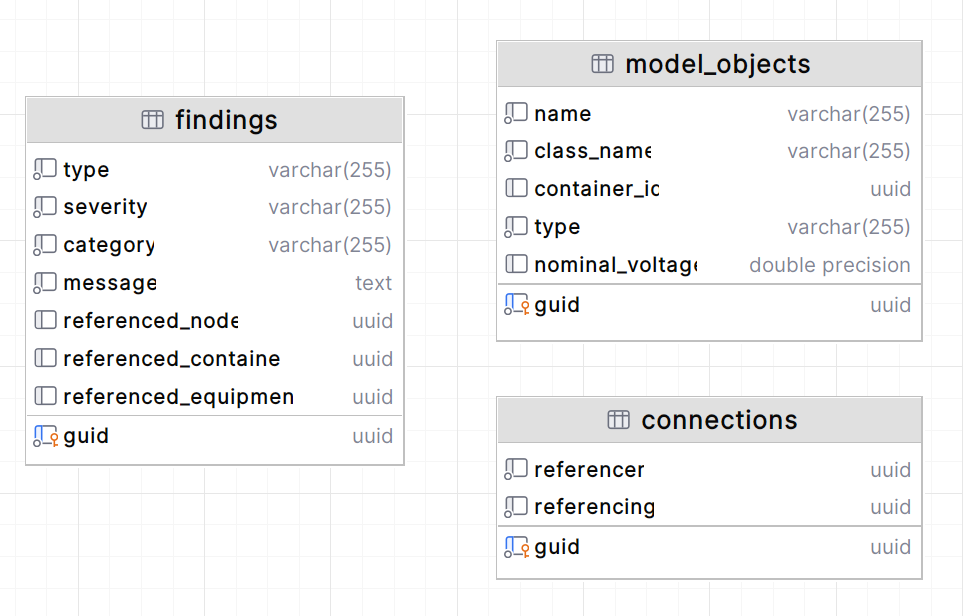
\includegraphics[width=0.9\textwidth]{content/img/Empire/Backend/tabellenstruktur.png}
    \caption{Tabellenstruktur des Prototyps}
    \label{fig:Tabellenstruktur}
\end{figure}
\FloatBarrier

\hspace{5em}